\section{Convolutional Autoencoders and U-Net}

\subsection{Convolutional Autoencoders (CAEs)}
As said, a Convolutional Neural Network processes structured grid data (like images) using a convolution operation defined by a kernel or filter. By sliding these filters across the image, CNNs naturally extract hierarchical features while drastically reducing the number of parameters compared to dense networks. \\
We can view a standard CNN as a powerful information compressor or encoder. In a classification task, a CNN processes an input image through successive convolutional and pooling layers until the spatial dimensions are severely compressed, finally feeding the extracted feature maps into a neural network (usually a MLP) to output class probabilities. If we remove the final NN classifier, we are left with a purely convolutional feature extractor. What if we try to decode this compressed representation back into the original image space? By attaching a \textit{convolutional decoder} to our \textit{convolutional encoder}, we create a \textbf{Convolutional Autoencoder (CAE)}. 

\begin{center}
    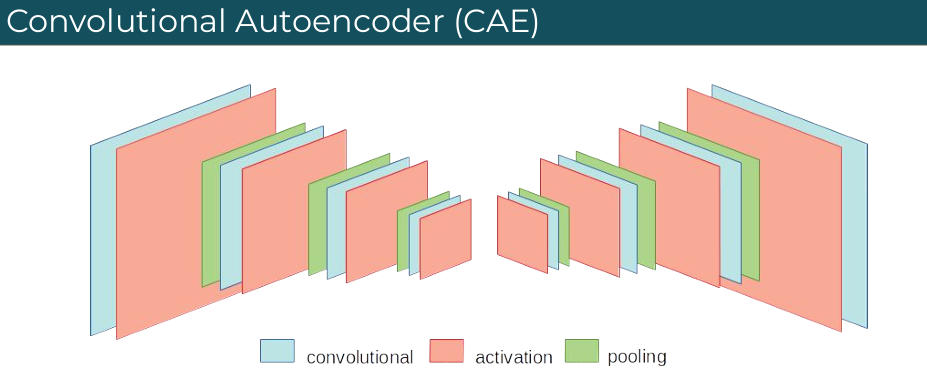
\includegraphics[width=0.75\textwidth]{figuresML_adv/lesson_ml_adv_2_pag_21.png}
\end{center}

\subsection{Upsampling and transposed Convolution in CAE}
In the encoder half of a CAE, pooling operations and strided convolutions are used to downsample the spatial dimensions of the image. That means that the latent space is no longer a simple 1D vector but a set of highly compressed, deep feature maps which constitute the latent representation of the data. To reconstruct the image in the decoder, we must invert this process and increase the spatial resolution of the feature maps.

\begin{figure}[H]
    \begin{minipage}[c]{0.55\textwidth}
        There are two primary ways to increase spatial resolution, as shown in the following figures:
        \begin{enumerate}
            \item \textit{Simple upsampling:} This is a fixed, non-learnable operation. It simply takes a pixel value and repeats it across a larger area. For instance, a $2 \times 2$ grid can be expanded to a $4 \times 4$ grid by duplicating each pixel into a $2 \times 2$ block. 
            \item \textit{Transposed convolution (Deconvolution):} Unlike simple upsampling, transposed convolution is a \textit{learnable} operation. It applies trainable filters to expand the spatial dimensions. For example, a single pixel in the compressed feature map is multiplied by a $2 \times 2$ filter (with a stride of 2), projecting its values into a $2 \times 2$ output grid. Where the projected outputs overlap, their values are summed. This allows the network to actively learn how to optimally reconstruct spatial details.
        \end{enumerate}
    \end{minipage}\hfill
    \begin{minipage}[c]{0.44\textwidth}
        \centering
        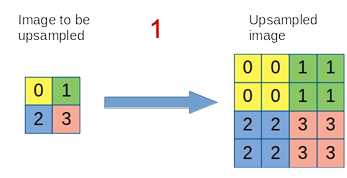
\includegraphics[width=0.85\textwidth]{figuresML_adv/lesson_ml_adv_2_pag_33.png}
        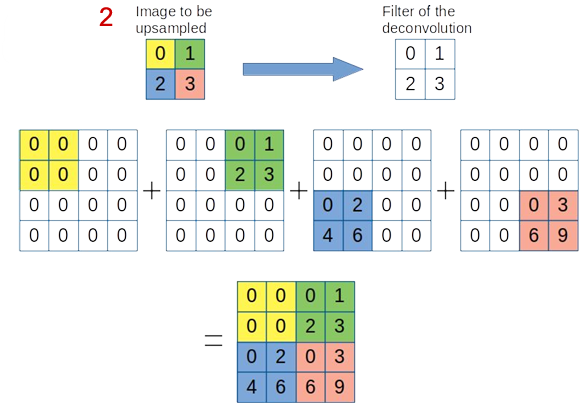
\includegraphics[width=0.85\textwidth]{figuresML_adv/lesson_ml_adv_2_pag_33a.png}
    \end{minipage}
\end{figure}
\vspace{-7.5mm}
With that said, it should be clear that CAEs are incredibly effective for unsupervised feature extraction. For example, take a look at the following study: \url{https://ieeexplore.ieee.org/document/7412749}. Here, Convolutional Sparse Autoencoders (CSAE) (a kind of CAE that introduces a sparsity penalty to force the most neurons to remain inactive for every given input) have been successfully used in medical imaging to extract features for breast density segmentation and mammographic risk scoring. The unsupervised CSAE isolates dense tissue structures without requiring pixel-perfect manual annotations, providing a foundation for subsequent supervised classifiers.

\subsection{Regularization in CNNs: spatial dropout}
Like any deep neural network, if a CAE has an excessively high capacity, it risks overfitting the training data. We must apply regularization techniques such as modifying the cost function with penalties, utilizing data augmentation, or applying batch normalization. 

A common regularization technique for MLPs is dropout, where random neurons are deactivated during training. However, applying standard dropout to CNN makes very little sense: in an image, adjacent pixels are highly correlated, so if you drop a single random pixel, the network can easily bypass the dropout by simply relying on the neighboring pixels, meaning the feature extractors can easily adapt to the change. To properly regularize a CNN, we use \textbf{spatial dropout}, a technique schematically reported in figure: instead of dropping individual random pixels, spatial dropout drops \textit{entire feature maps (channels) at random}. By completely zeroing out an entire filter's output for a given iteration, the network is forced to learn independent, robust feature representations rather than relying on a specific combination of parallel filters.

\begin{center}
    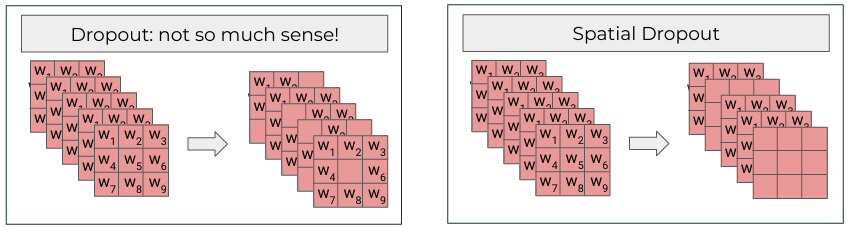
\includegraphics[width=0.85\textwidth]{figuresML_adv/lesson_ml_adv_2_pag_37.png}
\end{center}

\subsection{The U-Net architecture and skip connections}
Standard Convolutional Autoencoders suffer from a critical flaw when applied to highly detailed tasks like segmentation: the bottleneck compresses the image so severely that fine-grained spatial details (exact edges, boundaries, and microscopic structures) are permanently lost. The decoder struggles to reconstruct these sharp details from the low-resolution latent space alone.

To solve this, the \textbf{U-Net} architecture was introduced. U-Net is a fully convolutional neural network (which means it contains zero dense layers) featuring an encoder-decoder structure. It was implemented in 2015 for biomedical image segmentation of various organs, and it can still today be considered the state of the art architecture in its field. Its defining innovation is the use of the so called \textit{long skip connections}. Take a look at its structure in the following figure: as illustrated by the "U" shape of the architecture, the high-resolution feature maps from the early layers of the encoder are passed directly across the network and \textit{concatenated} with the upsampled feature maps in the decoder. 

\begin{center}
    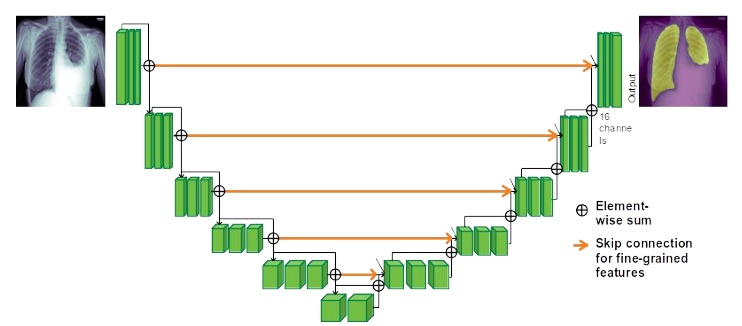
\includegraphics[width=0.85\textwidth]{figuresML_adv/lesson_ml_adv_2_pag_30.png}
\end{center}

We talked about skip connections in Sec. \ref{sec:skip_connections} regarding the ResNet algorithm and its functioning principle. Now let's take it a step further and distinguish between two different types of skip connections:
\begin{itemize}
    \item \textbf{Short Skip Connections} (e.g., ResNet, black lines in the figure above): Use element-wise \textit{addition} between closely grouped layers. Their primary purpose is to preserve information across depth and mitigate the vanishing gradient problem.
    \item \textbf{Long Skip Connections} (e.g., U-Net, orange lines in the figure above): Use \textit{concatenation} between the encoder and decoder. While they also reduce the vanishing gradient, their primary goal is to preserve high-resolution, fine-grained spatial features from the very first layers directly to the final reconstruction layers, bypassing the destructive compression of the bottleneck.
\end{itemize}

\subsection{Real life application: U-Net to assess COVID-19 pulmonary damage}

To fully grasp the importance and the mechanics of fully convolutional networks like the U-Net, it is extremely useful to look at a real-world application in the medical field. Medical images present unique challenges compared to standard natural image datasets (such as ImageNet). First, they are typically acquired at very high resolutions (e.g., a digital mammogram can be $4000 \times 4000$ pixels), and the diagnostic details we need to identify are often microscopic compared to the overall image size. Furthermore, a single 3D medical sample (like a computed tomography scan) can be massive, sometimes reaching several gigabytes in size. This completely prevents the standard approach of loading an entire dataset into a single array (e.g. in \texttt{NumPy}), as it would instantly exceed the memory limits of both the system RAM and the GPU.

A prominent example of overcoming these challenges is the development of automated software for the segmentation and quantification of COVID-19 lesions in CT scans, which was a critical necessity at the beginning of the pandemic. In COVID-19 pneumonia, there are two primary types of lung lesions: \textit{ground-glass} opacities (which are typically reversible) and \textit{consolidations} (which represent more severe and irreversible damage). Physicians needed a reliable way to quantify these lesions to assess the patient prognosis but a manual quantification on 3D CT scans is highly subjective and prone to severe inter-reader variability, especially for severely noisy images.

To solve this, researchers developed \textbf{LungQuant2.0}, a complex software architecture relying on a cascade of neural networks to provide reproducible, automated measurements. You can find the corresponding paper here: \url{https://arxiv.org/abs/2105.02566}. The pipeline (schematically represented below) operates as follows:
\begin{enumerate}
    \item[-] \underline{BBNet (Bounding Box Network):} The input CT scan is first processed by a simple 3D regression CNN. This network predicts the spatial coordinates of a bounding box enclosing the lungs, which is necessary to standardize the Field of View (FOV) across different patients and scanners.
    \item[-] \underline{U-Net$_1$ (lung segmentation):} The bounded region is fed into a first U-Net, which performs the precise semantic segmentation of the lung volume, separating the respiratory organs from the rest of the body.
    \item[-] \underline{U-Net$_2$ (lesion segmentation):} A second U-Net operates strictly within the isolated lung mask to segment the specific COVID-19 lesions, accurately classifying ground-glass opacities and consolidations.
\end{enumerate}

\begin{center}
    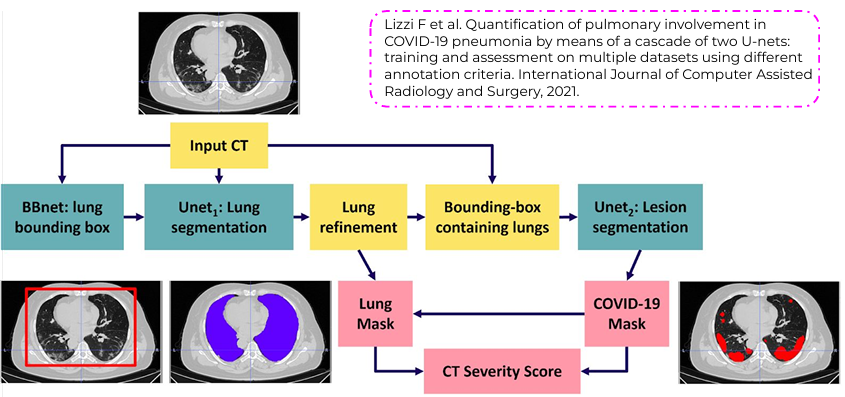
\includegraphics[width=0.85\linewidth]{figuresML_adv/lesson_ml_adv_2_pag_41.png}
\end{center}

The final output of this system provides physicians with crucial metrics, including the total lung volume, the CT Severity Score (CT-SS), and the precise volumes of the different lesion types in both the right and left lungs. 

\textbf{The critical importance of segmentation and explainability}

Working with real-world medical data highlights why aggressive segmentation (like the one performed by U-Net$_1$) is absolutely mandatory. Real datasets are rarely clean or perfect. During the COVID-19 emergency, patients with severe symptoms were often imaged directly in Intensive Care Units (ICUs) using portable, heterogeneous imaging systems. This resulted in extremely noisy images, sometimes with inverted color scales, where patients were poorly positioned and surrounded by external artifacts like breathing tubes, ECG cables, and hospital beds. 

In an initial phase of the study, researchers attempted to train a multi-input CNN to predict patient prognosis (severe vs. not severe) by feeding it raw, unsegmented chest X-Rays combined with clinical features (handling missing clinical data via k-nearest neighbors and mean imputation). The model achieved a seemingly excellent accuracy of around 75\%. 
    
However, when the \textit{Grad-CAM} (Gradient-weighted Class Activation Mapping) explainability algorithm was applied to visualize what the network was actually focusing on, the results were alarming. The network was completely ignoring the lungs. Because the dataset was highly biased by the emergency acquisition settings, the "smart" algorithm had learned to achieve high accuracy by looking at the background artifacts, such as the presence of ICU cables or the specific posture of a bedridden patient rather than analyzing the actual pulmonary pathology. 

This post-hoc explainability analysis perfectly demonstrated that without prior semantic segmentation, a CNN can easily "cheat" by learning confounding variables. By using a U-Net to strictly isolate the lungs and delete the irrelevant background, we force the subsequent classifier to base its predictions solely on genuine anatomical and pathological features.

%\begin{figure}[H]
%    \centering
%    \includegraphics[width=0.85\linewidth]{figuresML/image_5fedfc.png}
%    \caption{U-Net architecture details, dataset aggregation, and resulting case study correlations.}
%\end{figure}

\textbf{Practical implementation and training strategies}

Training these massive fully convolutional networks requires careful data management and specific architectural choices. Because we cannot load the entire dataset into memory, we must use \textbf{data generators}. A data generator dynamically loads small batches of images from the hard drive directly to the GPU during training. 

Furthermore, the generator is responsible for applying \textbf{real-time data augmentation}. By applying random transformations (rotations, zooms, elastic deformations) to the images on the fly, we regularize the network and prevent overfitting. While this approach saves an enormous amount of physical storage space since we do not need to save terabytes of pre-augmented images, it introduces a computational trade-off, as the CPU must spend time processing these transformations during the training loop.

Finally, to train the U-Net for medical segmentation, standard loss functions like MSE are often inadequate. Instead, custom differentiable loss functions must be explicitly programmed. A standard choice is the \textit{dice loss} (often combined with a weighted cross-entropy loss), which directly optimizes the volumetric overlap (volumetric Dice Similarity Coefficient, vDSC) between the predicted segmentation mask and the ground truth.

\subsection{Hands-on example on U-Nets}
To put these concepts into practice, the accompanying exercise involves building a U-Net of our own for lung segmentation. Due to the high memory requirements of processing large medical images, standard in-memory batching is insufficient. 
\begin{itemize}
    \item[-] We will implement a data generator to load batches of data dynamically and apply real-time data augmentation.
    \item[-] We will manually write the decoder path and the residual blocks of the U-Net, and implement the differentiable dice loss mathematically from scratch. 
\end{itemize}
Here is a general scheme of the project.

\begin{center}
    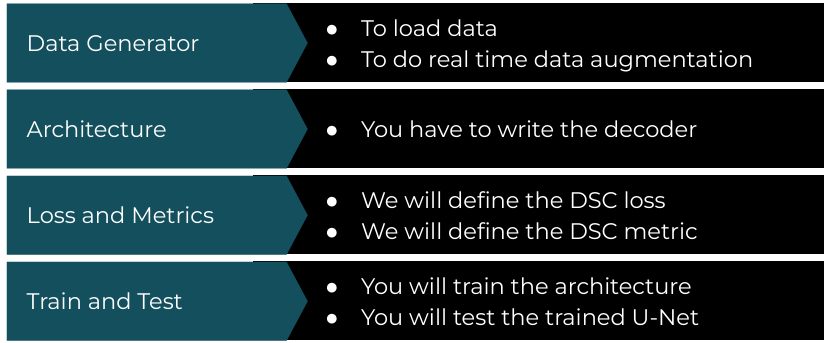
\includegraphics[width=0.6\linewidth]{figuresML_adv/lesson_ml_adv_2_pag_56.png}
\end{center}

Since I have to start a new page in order to input the Notebook in my LaTeX file, here is a photo of McEnroe and Borg taken before the 1980 Wimbledon final to occupy the rest of the page.

\begin{center}
    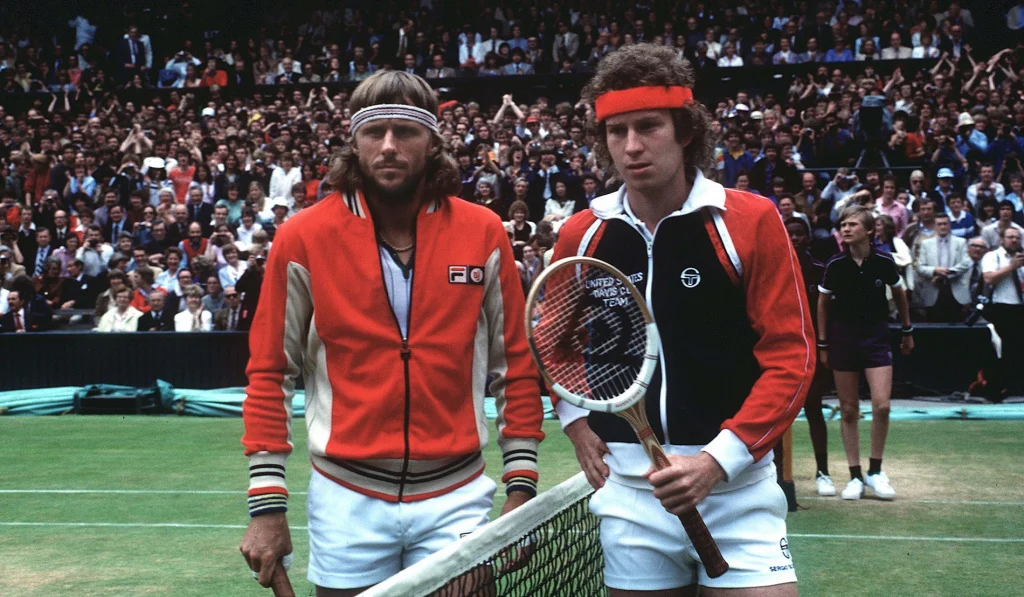
\includegraphics[width=0.4\textwidth]{figuresML_adv/borg_mcenroe_1980.png}
\end{center}

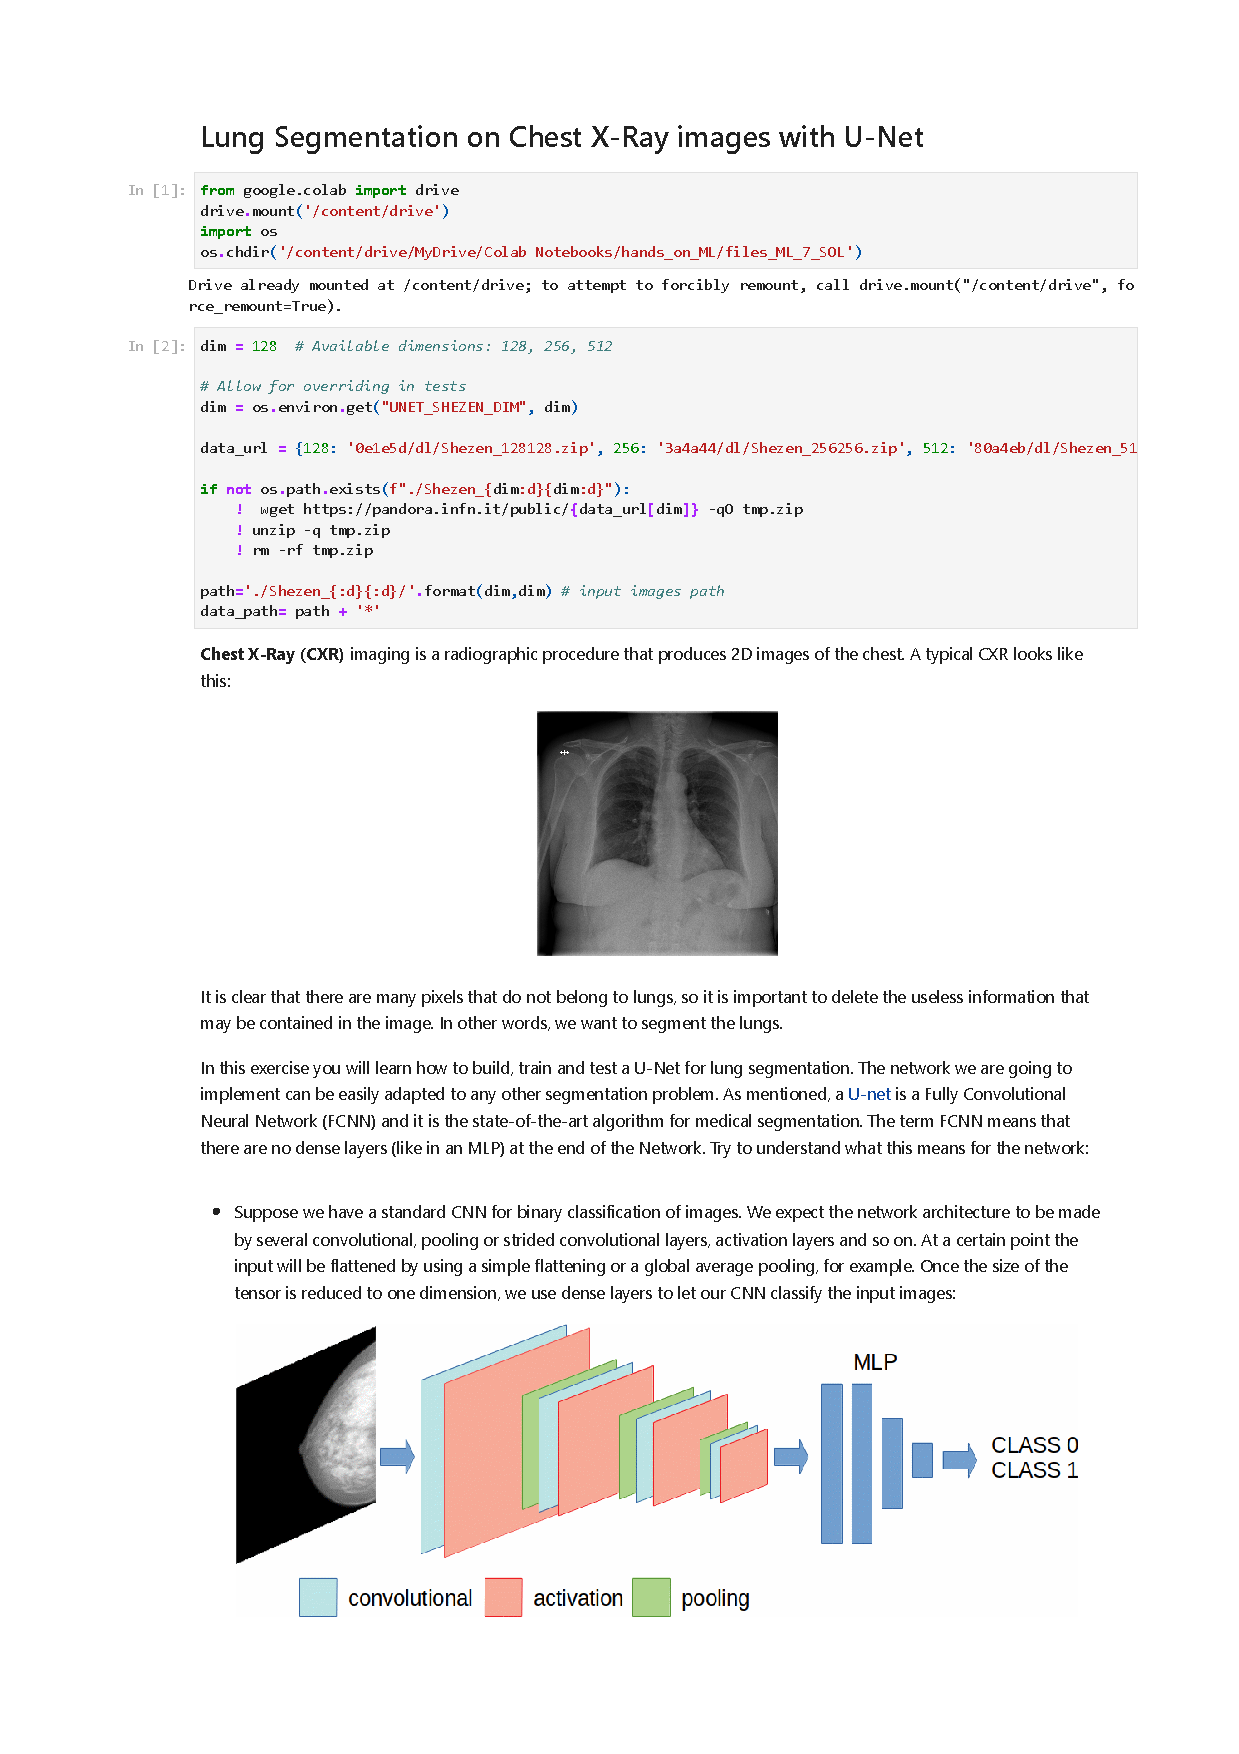
\includepdf[pages=-, pagecommand={\thispagestyle{plain}}]{lezioni/e_ML_adv_2hands_on.pdf} 
% ML_7 nel mio Colab

\begin{comment}
\subsection{Applications in Medical Imaging: LungQuant2.0}
Medical images possess unique challenges compared to standard datasets. They are often extremely high-resolution (e.g., $4000 \times 4000$ pixels) and require the identification of microscopic details. Furthermore, it is not always possible to process them patch-by-patch, making full-image segmentation essential to delete irrelevant anatomical parts from the field of view.

A practical application of U-Nets is the \textbf{LungQuant2.0} system, designed to quantify pulmonary involvement in COVID-19 pneumonia. The pipeline operates as a cascade of networks:
\begin{enumerate}
    \item \textbf{BBNet:} A 3D CNN regression model that predicts the 6 coordinates of the lung's bounding box to standardize the Field of View (FOV).
    \item \textbf{Unet$_1$:} A U-Net that receives the bounded CT scan and performs precise Lung Segmentation, outputting a clear Lung Mask.
    \item \textbf{Unet$_2$:} A subsequent U-Net that operates within the isolated lung mask to segment COVID-19 specific lesions (Ground Glass Opacities and Consolidations).
\end{enumerate}

To train these models, a combined loss function is utilized:
\begin{equation}
    L = \text{Dice}_{loss} + CE_{weighted}
\end{equation}
The loss combines the volumetric Dice Similarity Coefficient (vDSC) with a Weighted Cross-Entropy ($CE_{weighted}$) to heavily penalize errors on small, critical lesion areas. The output allows radiologists to automatically compute metrics like the CT Severity Score and precise lesion volumes.

\subsection{Real life application: U-Net to assess COVID-19 pulmonary damage}
To assess the overall prognosis of a COVID-19 patient, images alone may not be sufficient. We can build a \textbf{Multi-input Convolutional Neural Network} that combines categorical/continuous clinical features (e.g., Age, Temperature, WBC, PaO2, etc.) with Chest X-Ray images. The clinical data is pre-processed (using K-Nearest Neighbors imputation for missing variables and z-scoring), passed through dense layers, and subsequently concatenated with the flattened feature maps extracted from the CNN.

However, when deploying such models on noisy, real-world data (especially datasets acquired during emergency situations like the COVID-19 pandemic), we must verify what the network is actually "looking at". To do this, we use \textbf{Grad-CAM} (Gradient-weighted Class Activation Mapping), a post-hoc explainability algorithm that produces heatmaps highlighting the regions of the image most critical to the network's prediction.

As practically experienced in the lab, if we skip the U-Net lung segmentation step and feed the raw Chest X-Rays directly into the classifier, the network might achieve a deceptively high accuracy (e.g., 75\%). However, applying Grad-CAM reveals a critical flaw: the network is not looking at the lungs at all! Because the dataset is noisy and patients in severe conditions were often imaged in intensive care units with different equipment or poor positioning, the "smart" network learns to classify patient severity by recognizing external background artifacts (like tubes, cables, or image borders) rather than actual pulmonary pathology. \textit{This explicitly demonstrates why aggressive segmentation (via U-Net) to remove non-relevant data is absolutely mandatory in medical imaging.}

\subsection{Practical Exercise: U-Net for Lung Segmentation}
To put these concepts into practice, the accompanying exercise involves building a U-Net for lung segmentation. Due to the high memory requirements of processing large medical images, standard in-memory batching is insufficient. 
\begin{itemize}
    \item \textbf{Data Generators:} You will implement a Data Generator to load batches of data dynamically and apply \textit{real-time data augmentation}. Note that real-time augmentation introduces a trade-off: it saves storage space but heavily increases CPU/GPU computation time during training. 
    \item \textbf{Architecture \& Loss:} You will manually write the decoder path and the residual blocks of the U-Net, and implement the differentiable Dice Loss mathematically from scratch. 
\end{itemize}
\end{comment}